\documentclass[acmconf,nonacm=true]{acmart}
\authorsaddresses{}

% packages
\usepackage{float}
\usepackage{graphicx}
\usepackage{subcaption}
\usepackage[dvipsnames]{xcolor}
\usepackage{multirow}
\usepackage{enumitem}

\begin{document}
\title{ELEN0062 - Introduction to Machine Learning \\ 
Project 1 - Classification Algorithms}

% Enter your names here, along with your student IDs.
\author{Louis Hogge (\texttt{s192814})}
\author{Simon Louveau (\texttt{s194100})}
\author{Tom Weber (\texttt{s203806})}
% ordre alphabétique

\maketitle

\section{Decision Trees}

\begin{enumerate}
    \item \begin{enumerate}
        \item Here is an illustration of the decision boundary for each hyper-parameter value:
        \begin{figure}[H]
            \centering
            \begin{subfigure}[b]{0.5\textwidth}
                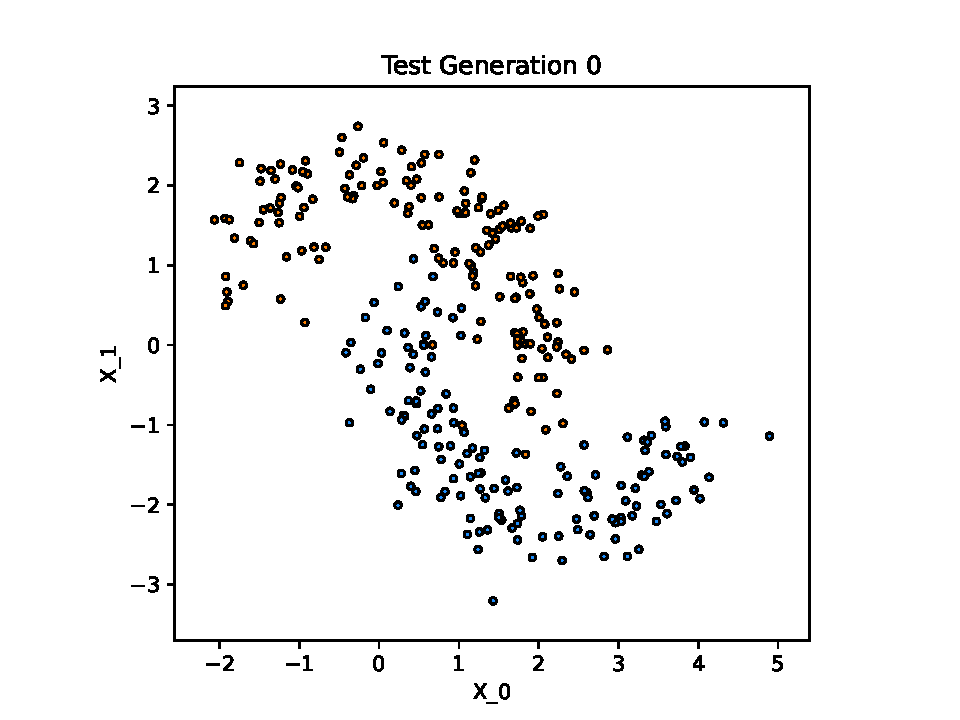
\includegraphics[width=\textwidth]{test_generation_0.pdf}
                \caption{Test Generation 0}
                \label{fig:test_generation_0}
            \end{subfigure}%
            \begin{subfigure}[b]{0.5\textwidth}
                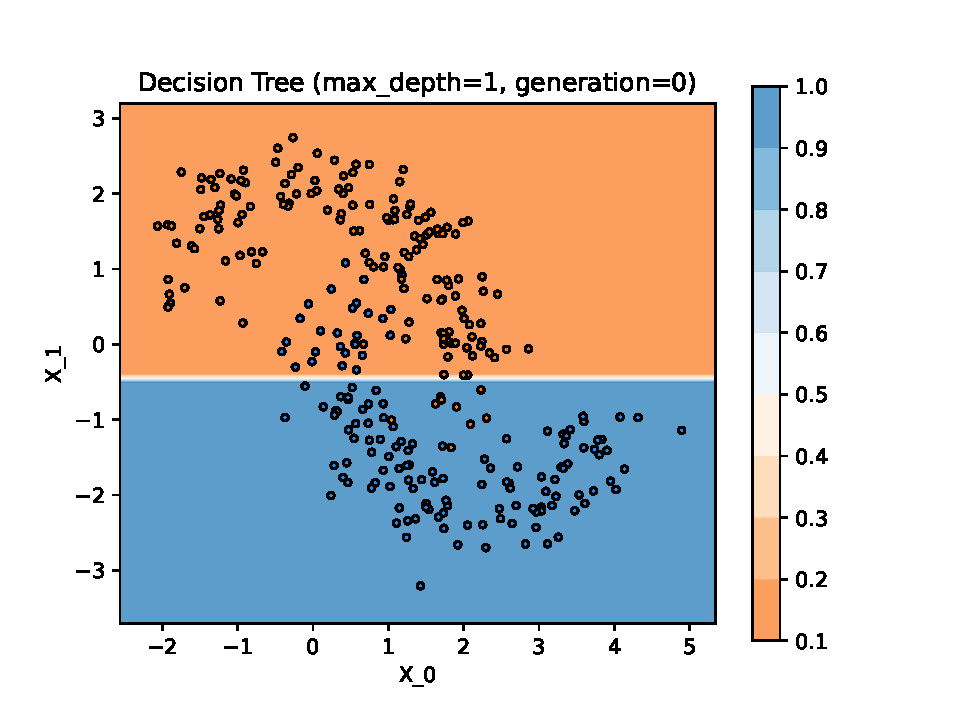
\includegraphics[width=\textwidth]{dt_depth_1_gen_0.pdf}
                \caption{Depth 1 Gen 0}
                \label{fig:dt_depth_1_gen_0}
            \end{subfigure}
            \label{fig:1.1_row_1}
        \end{figure}

        \begin{figure}[H]
            \centering
            \begin{subfigure}[b]{0.5\textwidth}
                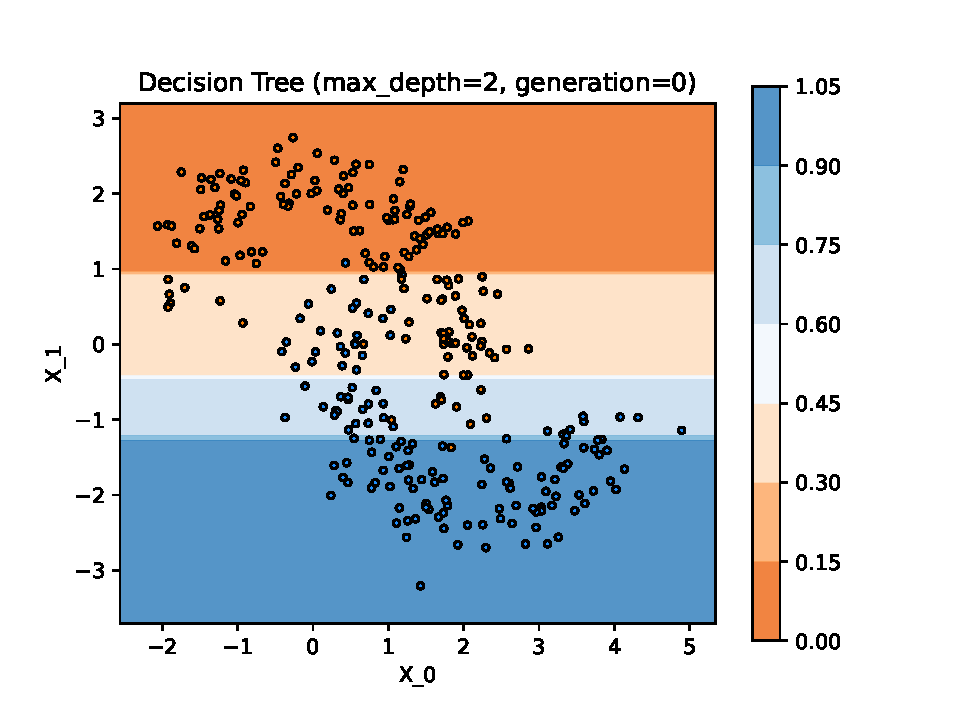
\includegraphics[width=\textwidth]{dt_depth_2_gen_0.pdf}
                \caption{Depth 2 Gen 0}
                \label{fig:dt_depth_2_gen_0}
            \end{subfigure}%
            \begin{subfigure}[b]{0.5\textwidth}
                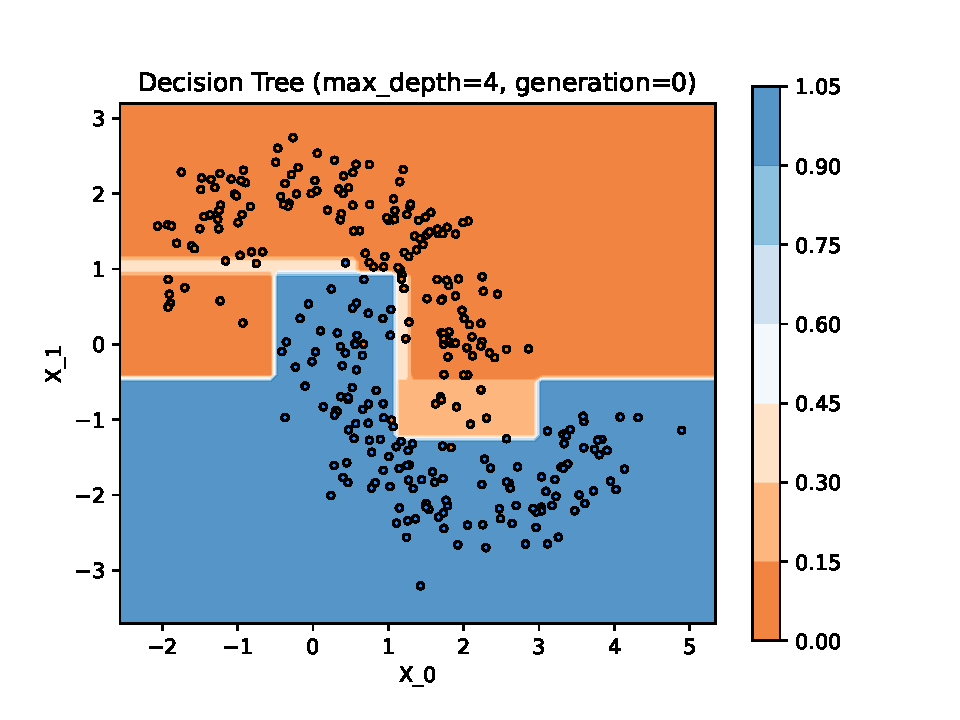
\includegraphics[width=\textwidth]{dt_depth_4_gen_0.pdf}
                \caption{Depth 4 Gen 0}
                \label{fig:dt_depth_4_gen_0}
            \end{subfigure}
            \label{fig:1.1_row_2}
        \end{figure}

        \begin{figure}[H]
            \centering
            \begin{subfigure}[b]{0.5\textwidth}
                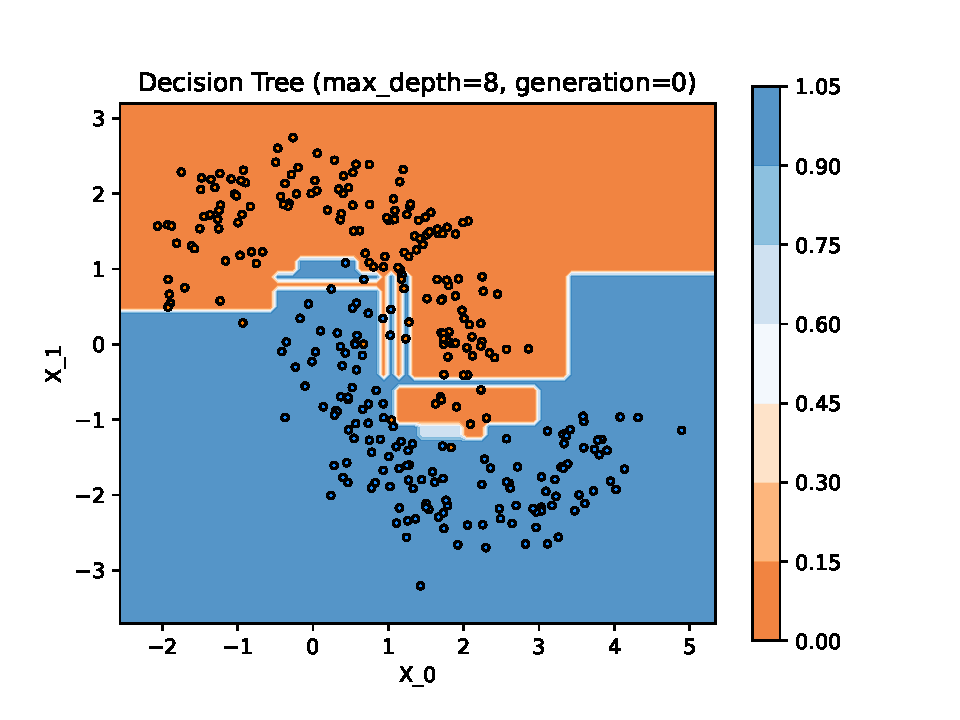
\includegraphics[width=\textwidth]{dt_depth_8_gen_0.pdf}
                \caption{Depth 8 Gen 0}
                \label{fig:dt_depth_8_gen_0}
            \end{subfigure}%
            \begin{subfigure}[b]{0.5\textwidth}
                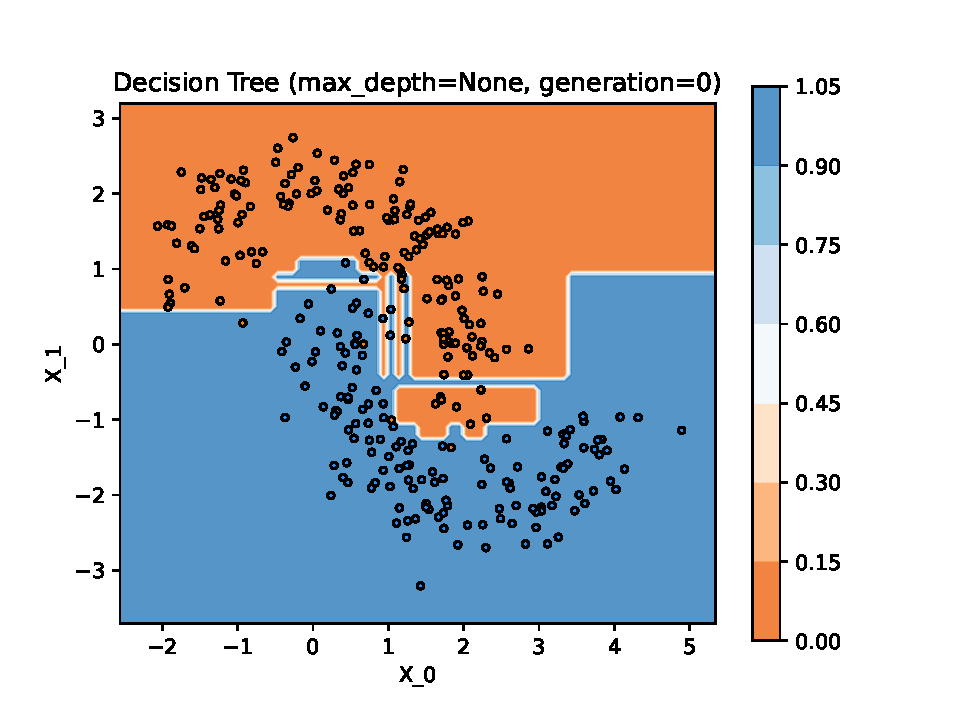
\includegraphics[width=\textwidth]{dt_depth_None_gen_0.pdf}
                \caption{Depth None Gen 0}
                \label{fig:dt_depth_None_gen_0}
            \end{subfigure}
            \label{fig:1.1_row_3}
        \end{figure}

        Here is an explanation of the decision boundary for each hyper-parameter value:
        \begin{itemize}
            \item \textbf{max\_depth \textit{1}:} With max\_dept \textit{1}, the decision tree makes only one decision split. The split in this model appears to be based on the x\_1 feature value. Data points above this line are predicted to belong to one class (represented by orange), and data points below are predicted to belong to another class (represented by blue). This type of simple decision boundary might not capture more complex patterns in the data.
            \item \textbf{max\_depth \textit{2}:} With max\_depth \textit{2}, the decision tree has the ability to implement up to three splits. The primary split is still founded on the x\_1 value, segregating the space into two principal areas. Two secondary splits further divide these primary zones, resulting in the emergence of a third and a forth distinct area. The orange region indicates one class, the middle light blue and light orange regions embodies areas where the model exhibits decreased confidence in its decision, and the blue region symbolizes a different class. The visual representation illustrates that some anomalies persist, particularly in the middle light blue and light orange zones.
            \item \textbf{max\_depth \textit{4}:} With max\_depth \textit{4}, the decision tree has the capacity to make multiple consecutive splits on the data. The dominant orange region at the top corresponds to one class, while the dominant blue region at the bottom represents another. Alternating spots of opposite color in these main regions (small blue pockets in the orange region and vice versa) highlight areas where the decision tree has identified more nuanced patterns and made exceptions to broader classifications.
            \item \textbf{max\_depth \textit{8}:} With max\_depth 8, the decision tree has the capability to make many more splits on the data, allowing it to recognize more intricate patterns. The visualization showcases the tree's efforts to account for nearly every deviation, even those that might be considered noise or outliers.
            \item \textbf{max\_depth \textit{None}:} With max\_depth \textit{None}, the decision tree is allowed to grow until it perfectly classifies all learning samples. This freedom can lead the tree to make numerous splits to distinguish between data points, making it exceptionally tailored to the learning set, it captures not just the underlying patterns but also the noise. As a result, the tree may not generalize well to new unseen data, the primary concern here being overfitting.
        \end{itemize}
        
        \item 
        \begin{itemize}
            \item \textbf{Underfitting:} Model with max\_depth \textit{1} \& \textit{2} are clearly underfitting. The decision boundaries of these models are relatively simplistic with only a few divisions: a single one for max\_depth \textit{1} and up to three for max\_depth \textit{2}. A significant number of data points are misclassified, the models fail to capture more complex patterns in the data.
            \item \textbf{Overfitting:} Model with max\_depth \textit{8} \& \textit{None} are clearly overfitting. For max\_depth \textit{None}, there's a highly detailed decision boundary that seems to bend around individual data points, especially in the regions of intricate blue and orange blend, max\_depth \textit{8} shows a similar trend but slightly less pronounced. Overfitting arises when the model tries too hard to capture not just the main patterns but also the noise or fluctuations in the test set. 
        \end{itemize}
        
        \item Because the confidence is inversely proportional to the proportion of the sample in a leaf and, when the max\_depth of a decision tree is set to its largest value or is unrestricted (i.e. max\_depth \textit{None}), the model can grow as deep as necessary to perfectly classify all learning instances. The tree will make very specific decisions tailored to the learning set resulting in small proportions of the sample in each leave.
    \end{enumerate}
    \item See table \ref{tab:avg_acc_std_dt}:
    \begin{table}[h]
    \centering
    \begin{tabular}{|c|c|c|}
        \hline
        \textbf{max\_depth} & \textbf{Average Accuracy} & \textbf{Standard Deviation} \\
        \hline
        \textit{1} & 0.8480 & 0.0236 \\
        \textit{2} & 0.8480 & 0.0236 \\
        \textit{4} & 0.9613 & 0.0117 \\
        \textit{8} & 0.9567 & 0.0145 \\
        \textit{None} & 0.9540 & 0.0136 \\
        \hline
    \end{tabular}
    \caption{average accuracy \& standard deviations for each max\_depth over five generations of the dataset}
    \label{tab:avg_acc_std_dt}
    \end{table}

    \begin{itemize}
        \item \textbf{max\_depth \textit{1} \& \textit{2}:}
        \begin{itemize}
            \item \textit{Average Accuracy:} Both max\_depth have the same average accuracy of 0.8480. This shows that increasing it from \textit{1} to \textit{2} doesn't improve the model's performance.
            \item \textit{Standard Deviation:} The standard deviation for both max\_depth is 0.0236, indicating a similar consistency in the model's performance across different generations of the dataset.
        \end{itemize}

        As we can see it in the illustrations provided in Q1(a), at these max\_depth, the model is underfitting the data. The model is too simple to capture the underlying patterns of the dataset, leading to suboptimal performance.

        \item \textbf{max\_depth \textit{4}:}
        \begin{itemize}
            \item \textit{Average Accuracy:} The average accuracy sees a significant jump to 0.9613, indicating that increasing the max\_depth to \textit{4} improves the model's ability to predict.
            \item \textit{Standard Deviation:} The standard deviation is 0.0117, which is lower than for max\_depth \textit{1} and \textit{2}. This means that model performance is more consistent than before between different generations of the dataset.
        \end{itemize}

        At a max\_depth of \textit{4}, the decision tree has a good balance between underfitting and overfitting, capturing the essential patterns of the data without becoming too specific to the learning data.

        \item \textbf{max\_depth \textit{8}:}
        \begin{itemize}
            \item \textit{Average Accuracy:} The accuracy is slightly lower than at max\_depth \textit{4}, coming in at 0.9567. This suggests that the model might be starting to overfit, becoming too tailored to the learning data and losing some ability to generalize.
            \item \textit{Standard Deviation:} The standard deviation increases slightly to 0.0145, hinting at a bit more variability in performance across dataset generations.
        \end{itemize}

        While the accuracy remains high, the slight drop coupled with the increased standard deviation suggests that the model might be capturing some noise or outliers, leading to overfitting.

        \item \textbf{max\_depth \textit{None}:}
        \begin{itemize}
            \item \textit{Average Accuracy:} The accuracy further decreases to 0.9540, reinforcing the notion that an unrestricted depth can lead to overfitting.
            \item \textit{Standard Deviation:} The standard deviation is 0.0136, which is between the values for max\_depth \textit{4} and \textit{8}, indicating a moderate consistency in performance.
        \end{itemize}

        Allowing the tree to grow unrestricted lead to a model that's overfitting. The model becomes too specific to the learning data, capturing noise and anomalies that don't generalize well to the test set.
    \end{itemize}
\end{enumerate}

\section{k-Nearest Neighbors}

\begin{enumerate}
    \item 
    Observe how the decision boundary is affected by the number of neighbors.
    \begin{enumerate}
        \item 
         Illustrate the decision boundary for each value of n\_neighbors:
         \begin{figure}[H]
            \centering
                \begin{subfigure}[t]{.495\textwidth}
                    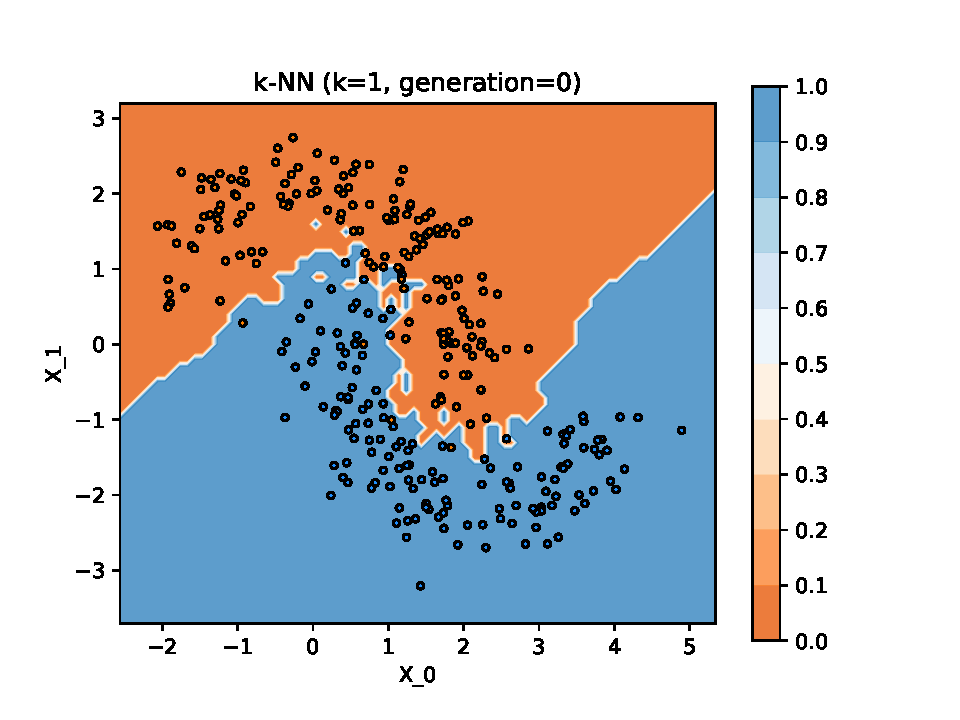
\includegraphics[width =1.2\textwidth]{knn_k_1_gen_0.pdf}
                    \caption{Decision boundary KNN k = 1}
                    \label{fig:knn_1}
                \end{subfigure}
                \hfill
                \begin{subfigure}[t]{.495\textwidth}
                    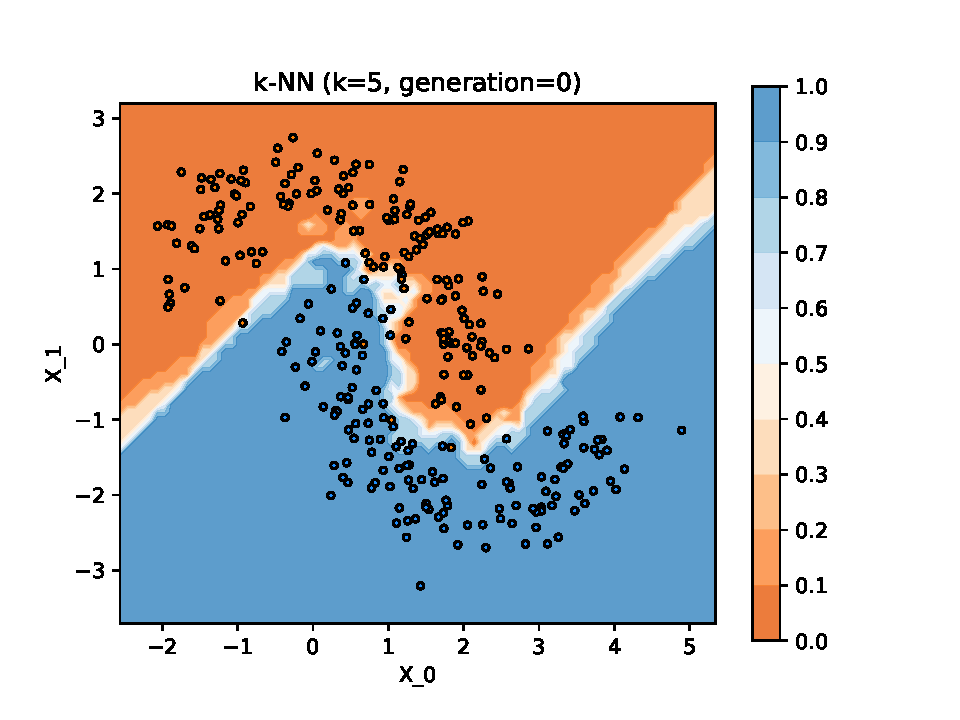
\includegraphics[width =1.2\textwidth]{knn_k_5_gen_0.pdf}
                    \caption{Decision boundary KNN k = 5}
                    \label{fig:knn_5}
                \end{subfigure}
            % \caption{Decision boundaries for KNN with k = 1 and k = 5}
            \label{fig:knn_1_5}
        \end{figure}
        
        \begin{figure}[H]
            \centering
                \begin{subfigure}[t]{.495\textwidth}
                    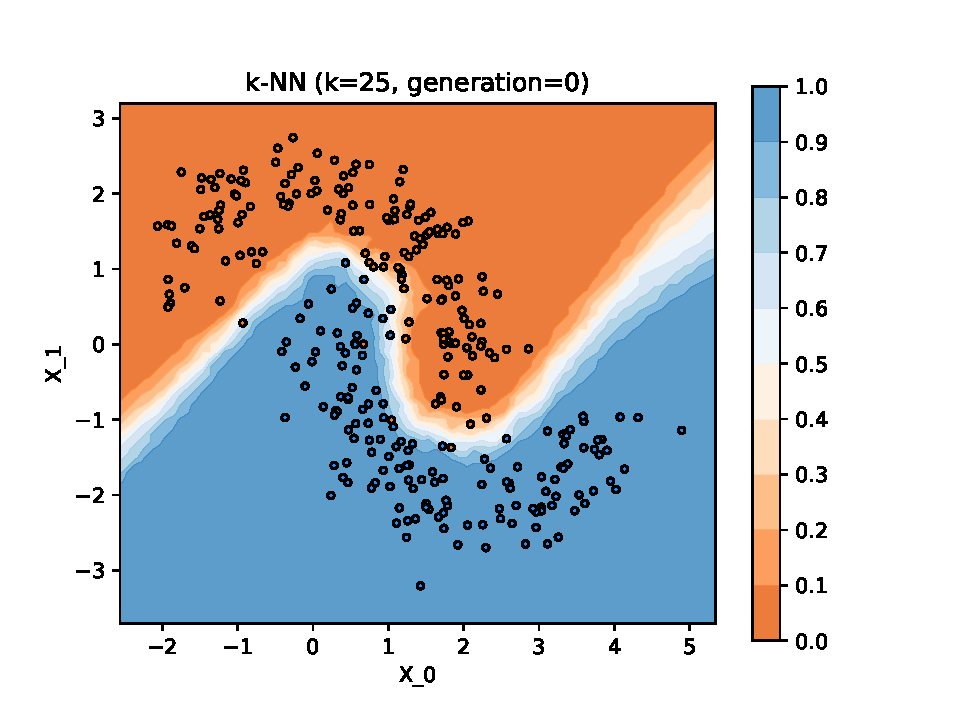
\includegraphics[width =1.2\textwidth]{knn_k_25_gen_0.pdf}
                    \caption{Decision boundary KNN k = 25}
                    \label{fig:knn_25}
                \end{subfigure}
                \hfill
                \begin{subfigure}[t]{.495\textwidth}
                    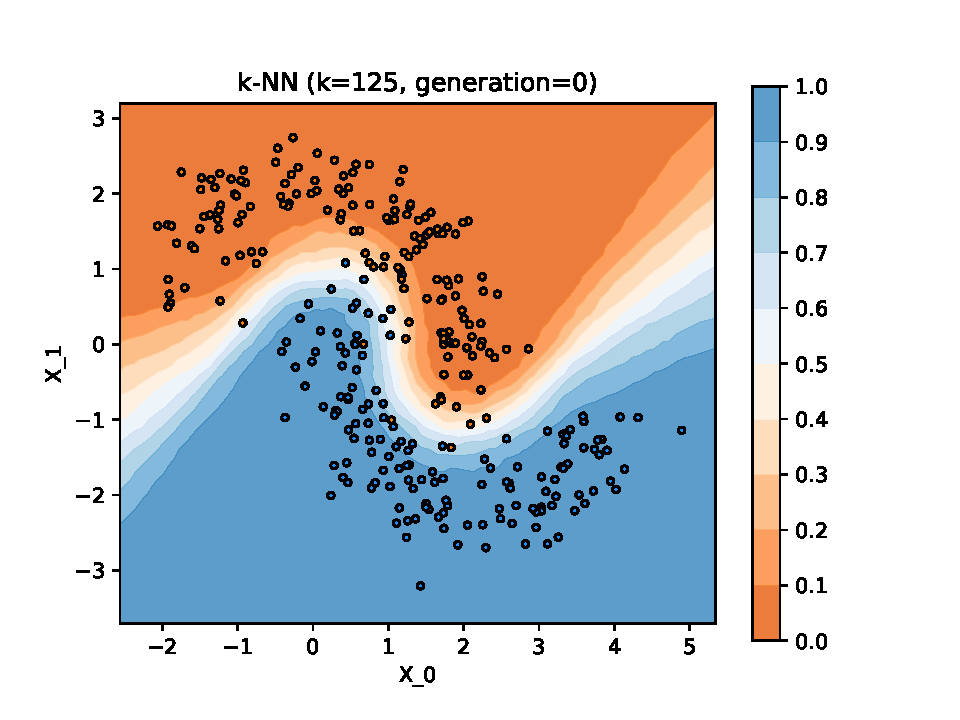
\includegraphics[width =1.2\textwidth]{knn_k_125_gen_0.pdf}
                    \caption{Decision boundary KNN k = 125}
                    \label{fig:knn_125}
                \end{subfigure}
            % \caption{Decision boundaries for KNN with k = 25 and k = 125}
            \label{fig:knn_25_125}
        \end{figure}
        
        \begin{figure}[H]
            \centering
                \begin{subfigure}[t]{.495\textwidth}
                    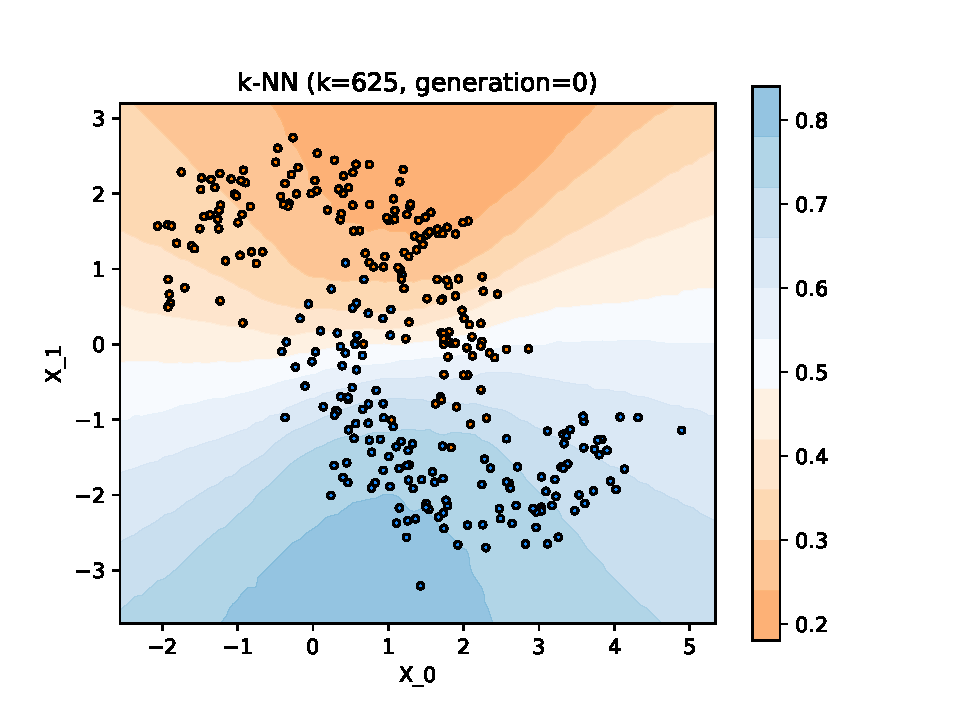
\includegraphics[width =1.2\textwidth]{knn_k_625_gen_0.pdf}
                    \caption{Decision boundary KNN k = 625}
                    \label{fig:knn_625}
                \end{subfigure}
                \hfill
                \begin{subfigure}[t]{.495\textwidth}
                    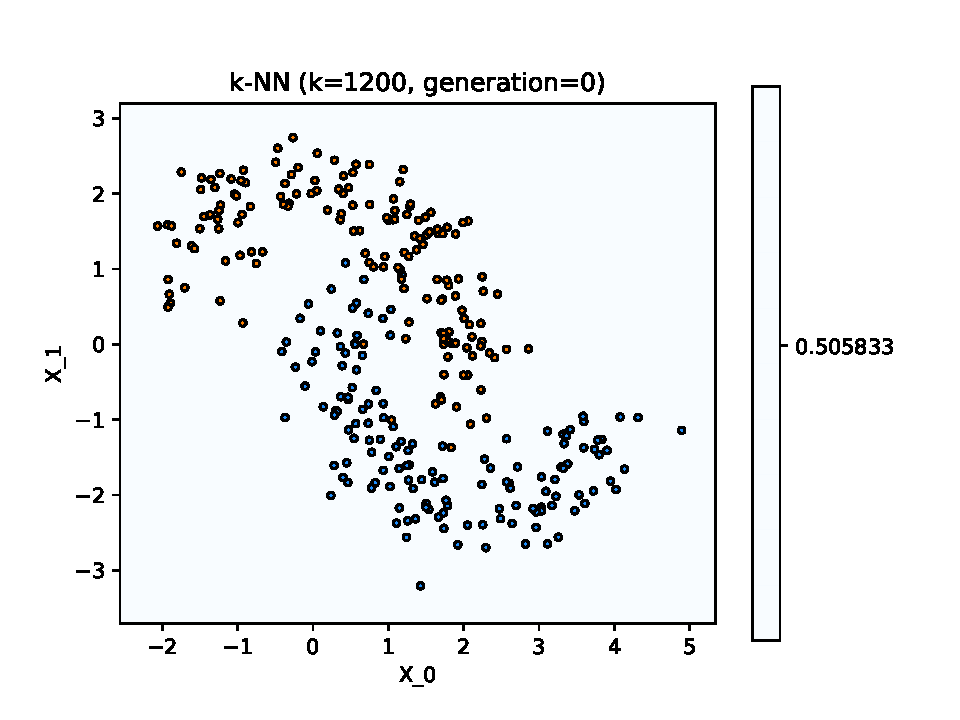
\includegraphics[width =1.2\textwidth]{knn_k_1200_gen_0.pdf}
                    \caption{Decision boundary KNN k = 1200}
                    \label{fig:knn_1200}
                \end{subfigure}
            % \caption{Decision boundaries for KNN with k = 625 and k = 1200}
            \label{fig:knn_625_1200}
        \end{figure}

     %     \begin{figure}[H]
    	% \centering
    	% 	\begin{subfigure}[t]{.495\textwidth}
    	% 		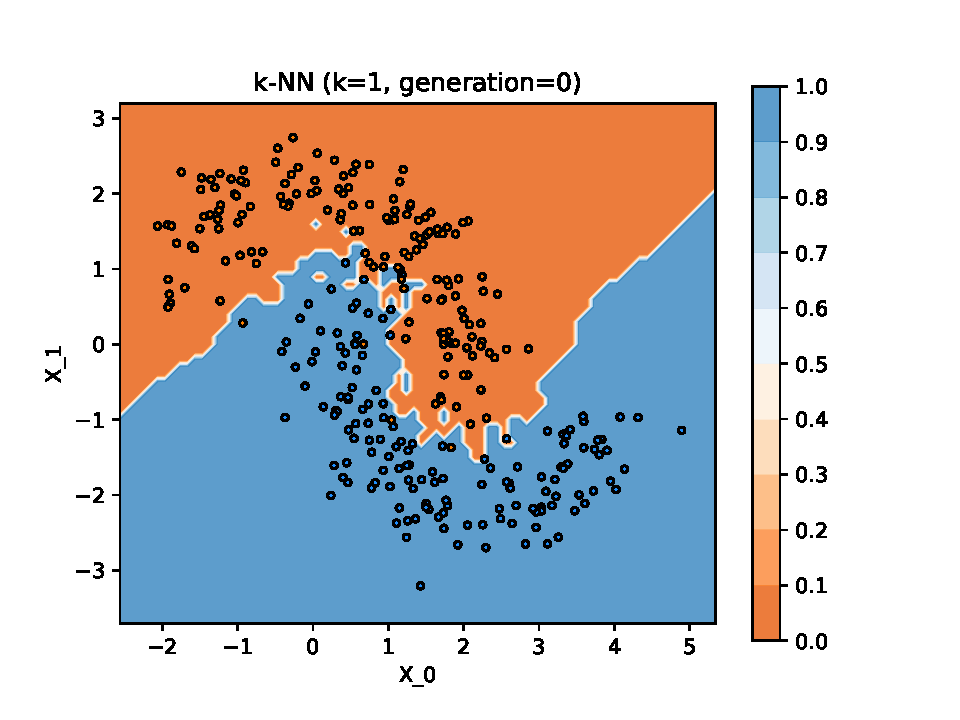
\includegraphics[width =1.2\textwidth]{knn_k_1_gen_0.pdf}
    	% 		\caption{Decison boundary KNN k = 1}
    	%         \label{fig:knn_1}
    	% 	\end{subfigure}
     %            \hfill
    	%     \begin{subfigure}[t]{.495\textwidth}
    	% 		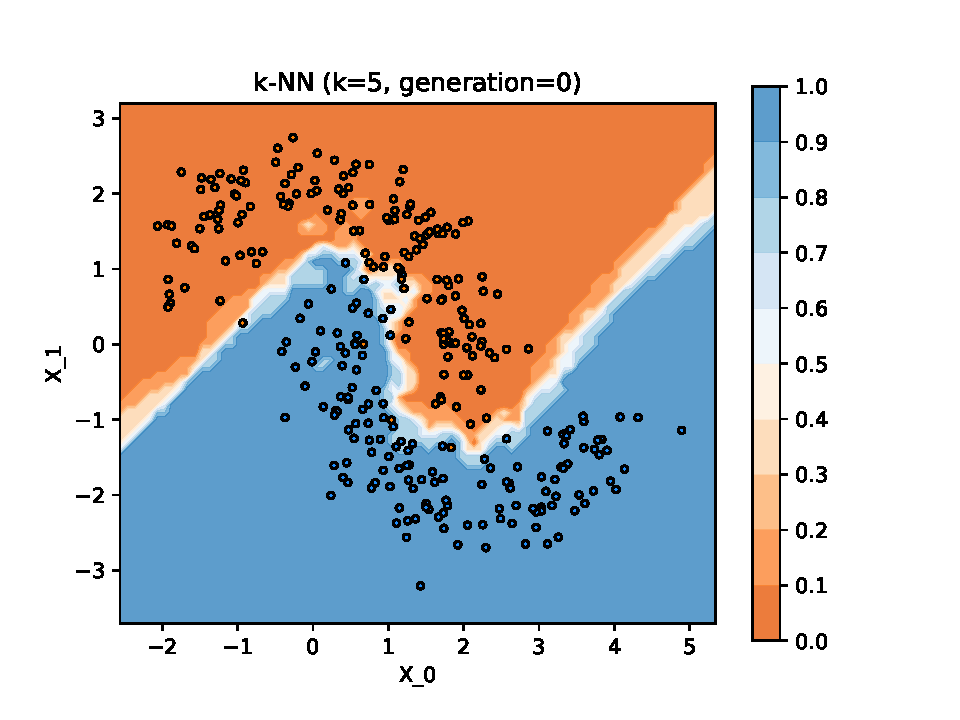
\includegraphics[width =1.2\textwidth]{knn_k_5_gen_0.pdf}
    	%         \caption{Decison boundary KNN k = 5}
    	%         \label{fig:knn_5}
    	% 	\end{subfigure}
    	% \label{fig:1.2}
     %       \hfill
    	% 	\begin{subfigure}[t]{.495\textwidth}
    	% 		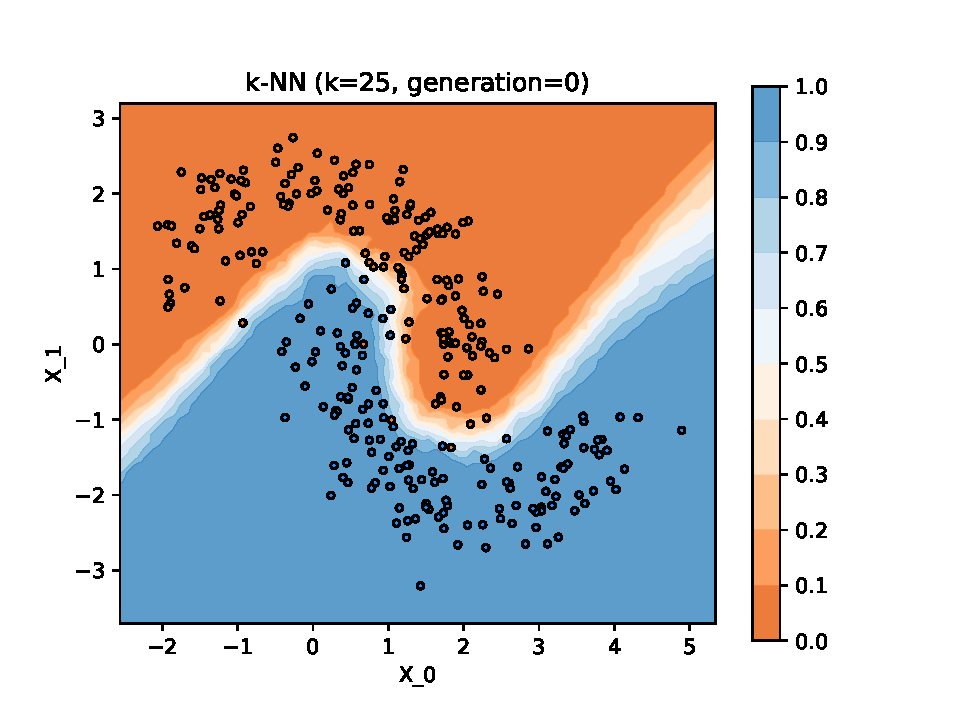
\includegraphics[width =1.2\textwidth]{knn_k_25_gen_0.pdf}
    	% 		\caption{Decison boundary KNN k = 25}
    	%         \label{fig:knn_25}
    	% 	\end{subfigure}
     %            \hfill
    	%     \begin{subfigure}[t]{.495\textwidth}
    	% 		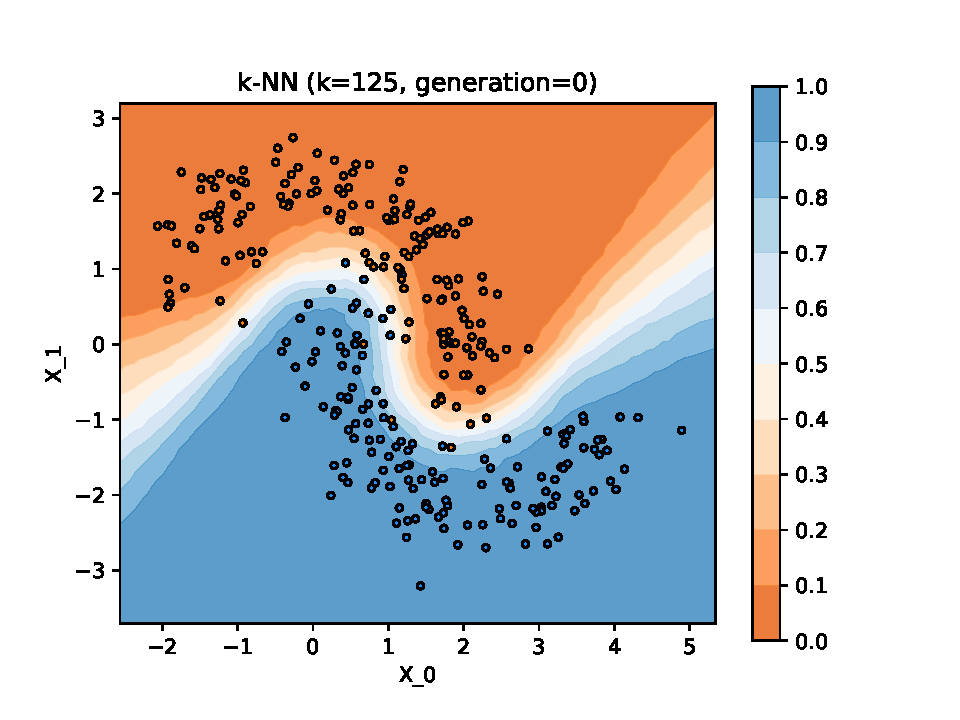
\includegraphics[width =1.2\textwidth]{knn_k_125_gen_0.pdf}
    	%         \caption{Decison boundary KNN k = 25}
    	%         \label{fig:knn_25}
    	% 	\end{subfigure}
    	% \label{fig:1.2}
     %    \hfill
    	% \centering
    	% 	\begin{subfigure}[t]{.495\textwidth}
    	% 		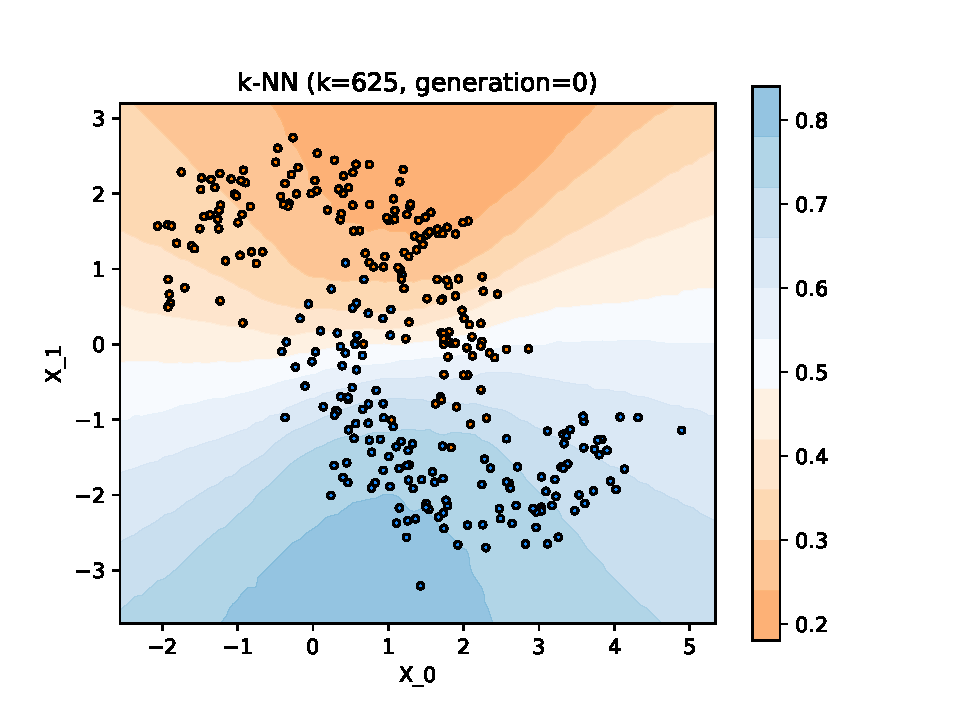
\includegraphics[width =1.2\textwidth]{knn_k_625_gen_0.pdf}
    	% 		\caption{Decison boundary KNN k = 625}
    	%         \label{fig:knn_625}
    	% 	\end{subfigure}
     %            \hfill
    	%     \begin{subfigure}[t]{.495\textwidth}
    	% 		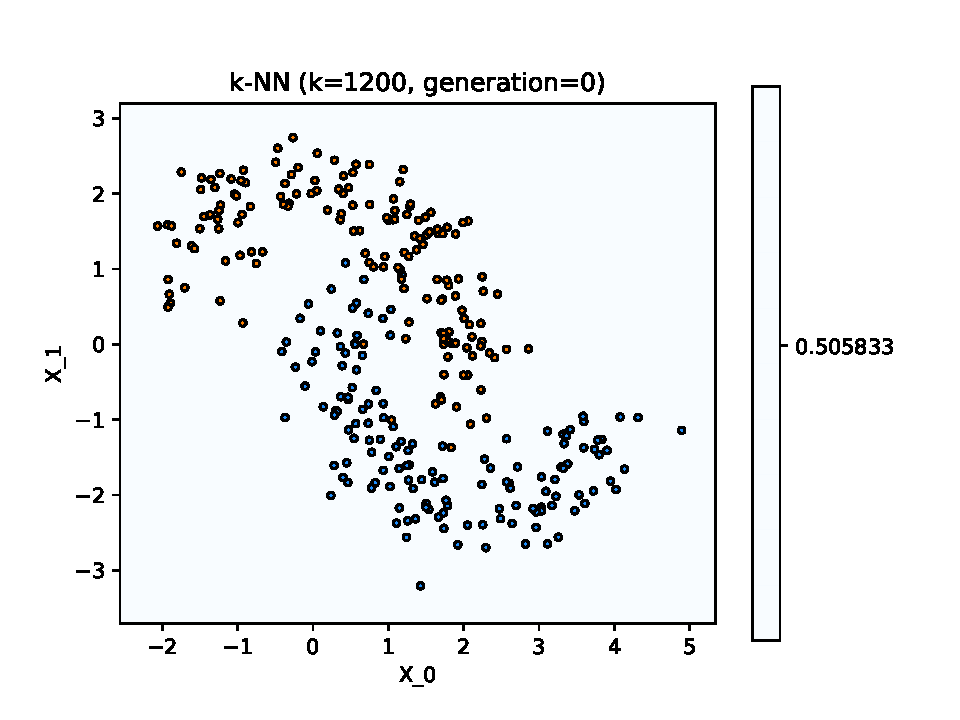
\includegraphics[width =1.2\textwidth]{knn_k_1200_gen_0.pdf}
    	%         \caption{Decison boundary KNN k = 1200}
    	%         \label{fig:knn_1200}
    	% 	\end{subfigure}
    	% \label{fig:1.2}
     %        \caption{Decision boundary computed for different value of k}
     %    \end{figure}
        \item 
        We can see on the following figures that the smaller the number of neighbors, the more overfitting (see Firgure \ref{fig:knn_1}). That is what we expected since a smaller number of neighbors means that the model will be very precise, and will overfit the data when reaching a k small enough. In the same way, if the number of neighbors is high, we expect the model to be less precise and therefore data will be underfitted, if \textbf{n\_neighbors} large enough (see Firgure \ref{fig:knn_625}). Of course if we take \textbf{n\_neighbors} equal to the size of the learning sample, then there will be only one class represented depending on which class has the most occurrences in the learning sample. The accuracy is then very low (visible on Figure [\ref{fig:knn_1200}], area is slightly orange because there is more occurancy in the learning sample).
    \end{enumerate}
    \item 
    The evolution of the decision boundary with respect to the number of neighbors. \\
    \begin{table}[h]
    \centering
    \begin{tabular}{|c|c|c|}
        \hline
        \textbf{n\_neighbors} & \textbf{Average Accuracy} & \textbf{Standard Deviation} \\
        \hline
        \textit{1} & 0.9513 & 0.0096 \\
        \textit{5} & 0.9647 & 0.0129 \\
        \textit{25} & 0.9660 & 0.0093 \\
        \textit{125} & 0.9660 & 0.0077 \\
        \textit{625} & 0.8420 & 0.0144 \\
        \textit{1200} & 0.4820 & 0.0113 \\
        \hline
    \end{tabular}
    \caption{average accuracy \& standard deviations for each n\_neighbors over five generations of the dataset}
    \label{tab:your_table_label}
    \end{table}
    \begin{itemize}
        \item \textbf{Average Accuracy:} \\
        - The average accuracy tends to improve initially as you increase 'k' because the algorithm is making decisions based on a larger and more representative group of neighbors, like we can see from k equals to 1 until 25 (even with 125 even it starts to decrease a bit). However, if 'k' becomes too large, it may lead to underfitting, where the model's performance drops again as it overly simplifies the decision boundaries, like it is clearly visible with 625 and 1200 where the average accuracy drops a lot.
        \item \textbf{Standard Deviation:} \\
         As 'k' increases, the model's predictions become more stable because it relies on a larger number of neighbors. This results in lower variance, and therefore, a smaller standard deviation in accuracy. However with $ k = 625$, it seems to always have a rise of the standard derivation. Considering the fact that after multiple simulation, the STD seems to decrease with $k$ unless with $k = 625$, I think at some point  the model is giving more weight to the potentially noisy neighbors, making the predictions more sensitive to such variations.
    \end{itemize}

    
\end{enumerate}

\section{Naive Bayes Classifier}

\begin{enumerate}
    \item 
    This section shows that the Naive Bayes (abbreviated NB) predictions $\hat{f}_{NB}-(\mathbf{x})$ under the assumption of independence, that is, input variables are conditionally independent given the output, can be obtained as such : $$\hat{f}_{NB}(\mathbf{x}) = \arg \max_{y}P(y)\prod_{i=1}^{p}p(x_{i}|y)$$ where P(y), the prior class probabilities can be estimated from class frequencies in the learning set, and the likelihood densities $p(x_{i}|y)$ are estimated as Gaussian densities : $p(x_{i}|y) = \frac{1}{\sqrt{2\pi\sigma^{2}_{i,y}}}exp(-\frac{(x_{i}-\mu_{i,y})^{2}}{2\sigma^{2}_{i,y}})$. \\Class-dependent mean $\mu_{i,y}$ and variance $\sigma^{2}_{i,y}$ can be estimated by the sample mean and variance, conditioned on the class.

    Thus, we want to show that under the hereabove independence assumption:
    \begin{equation} \label{eq:1}
    \hat{f}_{NB}(\mathbf{x}) = \arg \max_y P(y) \prod_{i=1}^{p} P(x_i|y)
    \end{equation}
    is equivalent to 
    \begin{equation} \label{eq:2}
    \arg \max_y P(y|x_1, \dots, x_p)
    \end{equation}
    
    Start from the Bayes Theorem, given class variable y and dependent feature vector $\mathbf{x}_{i}$ through $\mathbf{x}_{p}$:
    \begin{equation} \label{eq:3}
    P(y|x_1, \dots, x_p) = \frac{P(y) P(x_1, \dots, x_p|y)}{P(x_1, \dots, x_p)}
    \end{equation}
    
    Using the naive conditional independence assumption that :
    \begin{equation} \label{eq:4}
    P(x_{i}|y, x_1, \dots, x_{i-1}, x_{i+1}, \dots, x_p) = P(x_i|y)
    \end{equation}
    
    For all $i$, this relationship is simplified and allow to substitute this into the Bayes theorem formula :
    \begin{equation} \label{eq:5}
    P(y|x_1, \dots, x_p) = \frac{P(y) \prod_{i=1}^{p} P(x_i|y)}{P(x_1, \dots, x_p)}
    \end{equation}
    
   Since $P(x_1, \dots, x_p)$ is constant given the input :
   $$ P(y|x_1, \dots, x_p) \propto P(y) \prod_{i=1}^{p} P(x_i|y)$$

   We can then use the Maximum A Posteriori (MAP) estimation which is a Bayesian-based approach to estimate a distribution and model parameters that best explain an observed dataset :
   $$ \hat{f}_{NB}(\mathbf{x}) = \arg \max_y P(y) \prod_{i=1}^{p} P(x_i|y) = \arg \max_y P(y|x_1, \dots, x_p)$$

   Thus we have shown that Equation ~\ref{eq:1} is equivalent to ~\ref{eq:2} under our independence assumption.
   
    \item
    See file \( nb.py \) for the implementation :
    \begin{enumerate}
        \item[$\bullet$] Class NaiveBayesClassifier(BaseEstimator, ClassifierMixin)
        \begin{enumerate}
            \item[1.] def fit(self, X, Y)
            \item[2.] def gaussian\_density(self, x, mean, var)
            \item[3.] def predict(self, X)
            \item[4.] def predict\_proba(self, X)
            \item[5.] def predict\_log\_proba(self, X)
        \end{enumerate}
    \end{enumerate}
    \begin{figure}[h]
            \centering
            \begin{subfigure}[b]{0.5\textwidth}
                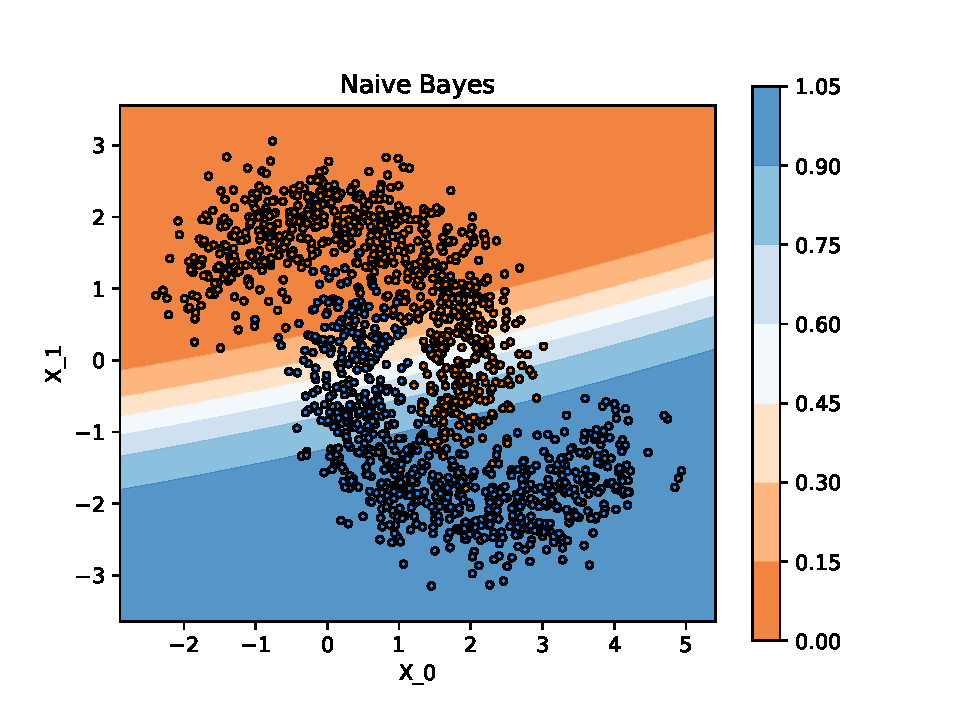
\includegraphics[width=\textwidth]{naive_bayes_nbg.pdf}
                \caption{Decision Boundary NB Learning Set}
                \label{fig:naive_bayes_nbg}
            \end{subfigure}%
            \begin{subfigure}[b]{0.5\textwidth}
                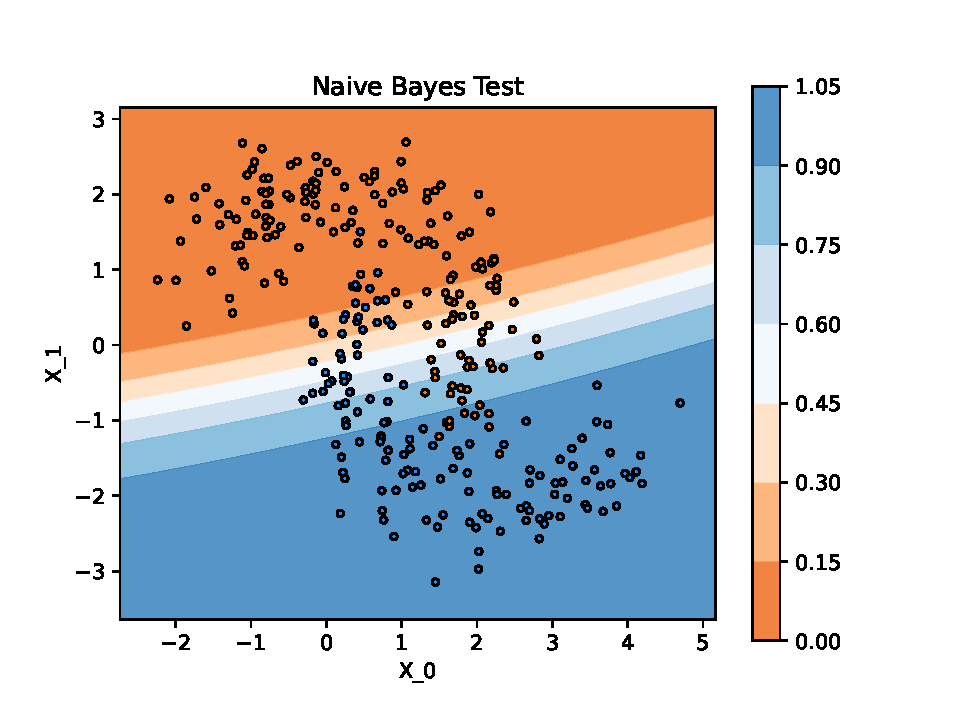
\includegraphics[width=\textwidth]{naive_bayes_test_nbg.pdf}
                \caption{Decision Boundary NB Test Set}
                \label{fig:naive_bayes_test_nbg}
            \end{subfigure}
            % \caption{Graphics Grouped by 2 - Row 3}
            \label{fig:grouped_by_2_row_3_simon}
        \end{figure}
    \item
    \begin{enumerate}
        \item[$\bullet$] LEARNING SET Figure \ref{fig:naive_bayes_nbg} : \\
        \textbf{Data points} are either blue or orange meaning it is a binary classification. The gradient shades of orange and blue, along with the white bands in between, represent the decisison boundaries and the probabilities associated with each class is in the colorbar. The deeper the shade, the higher the probability of a data point belonging to that particular class. \textbf{White bands} are areas of uncertainty where the classifier has roughly equal confidence in either class. Around the middle, there is a considerable overlap of orange and blue data points and this region is where the classifier has a higher misclassification rate. The decision boundaries appear to be linear but still a bit curved. Knowing the fact that the dataset is the make\_moon dataset from scikit-learn, it provides additional context. The "moons" create a non-linear pattern as we can see an overlap of the two moons in the middle. This makes it hard for the classifier especially in our case. We used the Gaussian Naive Bayes, where each feature is assumed to be normally (Gaussian) distributed. If we assume a Gaussian Naive Bayes, then the likelihood of the features given the class is modeled as a Gaussian distribution bringing non-linear characteristics.

        \item[$\bullet$] TEST SET Figure \ref{fig:naive_bayes_test_nbg} : \\
        \textbf{Data points} and decision boundaries are the same as it was for the learning set. We can also see misclassified data points (orange points in the deeper blue region and vice versa) in the boundary regions where the classifier transitions from one class to another.
        \textbf{The overlapping region} is still challenging for our classifier.
        One thing that is important is the fact that the decision boundaries appear consistent with what was observed with the learning set meaning that the classifier has generalized its decision boundaries and is not overfitting to the learning data. However, the problem linked with the fact that linear decision boundaries can't capture complex nonlinear relationships between features and class labels is still present and the white region remains a high misclassification region.
    \end{enumerate}
    \item See table \ref{tab:accuracy_sd_nb}: \\
    Accuracy can appear to be good but there is room for improvement and the standard deviation shows that there is variability ! 
    \begin{table}[h]
    \centering
    \begin{tabular}{|c|c|c|}
        \hline
        \textbf{Generations of data} & \textbf{Average Accuracy} & \textbf{Standard Deviation} \\
        \hline
        \textit{5} & 82.60\% & 1.53\% \\
        \hline
    \end{tabular}
    \caption{average accuracy \& standard deviations for Gaussian Naive Bayes}
    \label{tab:accuracy_sd_nb}
    \end{table}
\end{enumerate}

\section{Method Comparison}

\begin{enumerate}
    \item We use GridSearchCV to conduct an exhaustive search over a predefined range of hyperparameter values, specifically focusing here on \textit{max\_depth} for decision trees and \textit{n\_neighbors} for k-NN. Initially, a parameter grid is defined, where the keys are the parameter names (\textit{max\_depth} \& \textit{n\_neighbors}) and the values are lists of settings we wish to explore (\textit{max\_depth = 1, 2, 4, 8, None} \& \textit{n\_neighbors = 1, 5, 25, 125, 625}).\\
    
    GridSearchCV operates by evaluating all possible combinations of the specified hyperparameters to identify the combination that yields the optimum performance, as determined here by accuracy.\\
    
    This is achieved through k-fold cross-validation on the learning set. In k-fold cross-validation, the learning set is partitioned into k subsets. The model is trained on k-1 subsets and validated on the remaining subset, cycling through so that each subset serves as the validation set exactly once. This process is repeated for every unique combination of hyperparameters in the grid.\\
    
    Upon completion, GridSearchCV provides the best hyperparameter values found during the search. We then utilize these optimal values to train the models on the entire learning set. After that, the performance of the models is evaluated on the test set.\\
    
    An important limitation to note is the scenario when attempting to run GridSearchCV for the k-NN model with k=1200, given that the size of the learning set is also 1200. When performing k-fold cross-validation with 5 subsets (as it is done in our code), the training process for each fold involves using 4 of these subsets, while the remaining subset is used for validation. The combined size of the 4 subsets used for training is 960, as each subset contains 240 observations (since 1200/5 = 240), and thus 240*4 = 960. This situation illustrates a constraint where the specified k value for the k-NN model exceeds the size of the training set available during cross-validation. The problem remains the same whatever the choice of the number of subsets to be used for k-fold cross-validation.\\
    \item See table \ref{tab:avg_acc_std_tuning}:
    \begin{table}[H]
        \centering
        \begin{tabular}{|l|c|c|}
            \hline
            \textbf{Model} & \textbf{Average Test Accuracy} & \textbf{Standard Deviation} \\
            \hline
            Decision Tree & 0.9633 & 0.0110 \\
            k-NN & 0.9680 & 0.0102 \\
            \hline
        \end{tabular}
        \caption{average accuracy \& standard deviation for Decision Trees and k-NN models over five generations of the dataset}
        \label{tab:avg_acc_std_tuning}
    \end{table}

    Note that:

    \begin{table}[h]
        \centering
        \begin{tabular}{|c|c|c|}
        \hline
        \textbf{Model} & \textbf{Generation} & \textbf{Best Hyperparameter} \\
        \hline
        \multirow{5}{*}{Decision Tree (Max Depth)} & Gen 0 & 4 \\
         & Gen 1 & 4 \\
         & Gen 2 & 4 \\
         & Gen 3 & 8 \\
         & Gen 4 & 4 \\
        \hline
        \multirow{5}{*}{k-NN (N Neighbors)} & Gen 0 & 25 \\
         & Gen 1 & 25 \\
         & Gen 2 & 25 \\
         & Gen 3 & 25 \\
         & Gen 4 & 5 \\
        \hline
        \end{tabular}
        \caption{Best hyperparameters for Decision Tree and k-NN across different generations}
        \label{tab:hyperparameters}
    \end{table}

    \item
    Both the Decision Tree and K-Neighbors classifiers outperform the Naive Bayes classifier on this dataset as we can see on this Table \ref{tab:avg_acc_std_comp}.

    \begin{table}[H]
        \centering
        \begin{tabular}{|l|c|c|}
            \hline
            \textbf{Model} & \textbf{Average Test Accuracy} & \textbf{Standard Deviation} \\
            \hline
            Decision Tree & 96.33\% & 1.10\% \\
            k-NN & 96.80\% & 1.02\% \\
            Naive Bayes &  82.60\% & 1.53\% \\
            \hline
        \end{tabular}
        \caption{average accuracy \& standard deviation for Decision Trees, k-NN and naive Bayes models over five generations of the dataset}
        \label{tab:avg_acc_std_comp}
    \end{table}

    \begin{itemize}
        \item 
        The average accuracy of the DT and k-NN is significantly higher than that of the Naive Bayes classifier. This suggests that the 2 first algorithms are better at correctly classifying instances from this dataset than NB which is normal because the dataset has non-linear properties (\textbf{make\_moons()}) \label{disadv_nb} [3].

        \item 
        The standard deviation, which measures the amount of variation in the accuracy results, is also lower for the DT and k-NN compared to the Naive Bayes. This indicates that the performance of those two is more consistent across different runs.
        
        \item
        The performance of these classifiers can be influenced by many factors, including the characteristics of the dataset (number of instances, number of features, noise level)
        
        \item 
        We have decide to rank these algorithms based on the average accuracy and the standard deviation even if the Naive Bayes model is disadvantaged like said above [\ref{disadv_nb}] . So between the Decision Tree and k-NN, the K-Neighbors classifier has a slightly higher average accuracy and a slightly lower standard deviation, making it the best performing model among the three. \\
        However, we do not forget that the Naive Bayes model has some advantages compared to the others but it is not reflected in our criteria like :
        \begin{enumerate}
            \item 
            \textbf{Simplicity and Speed:} Naive Bayes is a relatively simple algorithm based on conditional probability and counting, and it’s often faster during both training and prediction phases than more complex models like k-NN (slower in prediction phase) or Decision Trees (slower in training phase).

            \item 
            \textbf{Ease of Implementation:} The Naive Bayes algorithm is straightforward to implement and understand.

            \item 
            \textbf{Performance with High-Dimensional Data:} Naive Bayes can perform well with high-dimensional data. In cases where the number of features is very large, Naive Bayes can often outperform more complex models like k-NN which is sensitive to the size of the dataset and high-dimensional  can lead to a significant increase in distance calculations .
        \end{enumerate}
        
        
        \item 
        In conclusion, based on these results, the ranking of the methods on this dataset would be:
        
        
        \begin{enumerate}[label=\arabic*)]
            \item 
            K-Neighbors (with GridSearchCV for hyperparameter tuning)
            
            \item 
            Decision Tree (with GridSearchCV for hyperparameter tuning)
            
            \item 
            Naive Bayes.
    
        \end{enumerate}
        
    \end{itemize}
    
\end{enumerate}

\end{document}